\chapter{Bluetooth Performance}
In order to better understand how much performance could be expect from Bluetooth in real-world conditions two benchmarks were implemented to simulate different scenarios.
The first scenario being simulated was the transmission of a large payload, such as a picture or video to another device while the second benchmark focused on the delivery of smaller payloads such as text messages, to multiple devices.

\section{Devices}
Different devices were employed for testing. Table \ref{table:devices-used} provides a correspondence between names used in the graphs and the mark and model of the devices used.

\begin{table}[h]
\centering
\caption{Devices used for performance test}
\label{table:devices-used}
\begin{tabular}{lllll}
\hline
Name        & Manufacter        & Model name    \\ \hline
Nexus 5     & Google            & Nexus 5       \\
Nexus 7     & Google            & Nexus 7       \\
OnePlus One & OnePlus           & One           \\
Redmi       & Xiaomi            & Redmi 2       \\ 
\hline
\end{tabular}
\end{table}

\section{Benchmark Application}
All of the benchmarking code was implemented in a standard android application which is available on Github \cite{benchmarking-code}.
The application was responsible for running a simulation and collecting the relevant metrics for each simulation scenario.
To allow programmatic access to all this functions, a small HTTP server \cite{nanohttpd} was embedded into the application.
This approach allowed manual testing of the functionality during development as well as allowing a remote script to run the real simulations.
Three endpoints were exposed on the HTTP server by the application; one to get the Bluetooth name and MAC address of the device and two to run simulations.
A python script was developed to run the individual simulations, collect and plot the data generated in the process.
The script used the list of local IP addresses as input and collected all of the necessary information via the \texttt{/mac} HTTP endpoint on each device.

\section{Throughput}
The throughput benchmark was designed to test the performance of RFCOMM connections between two devices ``A'' and ``B''.
In this scenario one of the two devices was tasked with being the server while the other performed the benchmark and sent the results back to the HTTP client.
To initiate a test the script invoked the \texttt{/throughput?target=<mac>} endpoint on the client device passing the Bluetooth mac address of the target as a parameter.
At this point a RFCOMM connection was established between the client and the server and the server started to send messages to the client.
The time to receive each message was computed by the client for each message.
The connection was closed by the client after 10 messages were received.
A CSV containing each measurement was sent back as a response to the HTTP request.
The CSV contained four columns: ``from'', ``to'', ``size'' and ``time''.
``from`` and ``to'' contained the Bluetooth mac address of the client and the server respectively, ``size'' contained the size of the packet and ``time'' contained the elapsed time for each message in nanoseconds.

The benchmark was run between each pair of devices and the results obtained are shown in Figure \ref{figure:throughput}.
The names on the top of the graph are the servers and on the bottom are the clients. 

\begin{figure}[ht!]
  \centering
  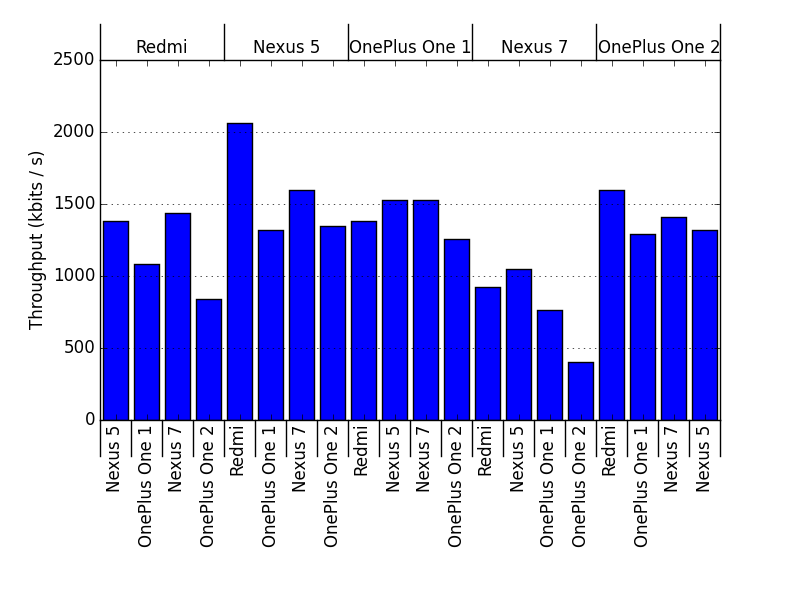
\includegraphics[width=1.0\textwidth]{img/throughput.png} 
  \caption{Throughput}
  \label{figure:throughput}
\end{figure}



\section{Raw Throughput}

??

\section{Messages per second}
The second benchmark was designed to test the ability of a device to send multiple messages to a variety of other devices.
The test consisted in a device, the master, that sent a multitude of messages to a set of devices, which then sent a response for each message received from the master.

To initiate the test the script invoked the \texttt{/messages} endpoint on the master device, sending a list of targets and the number of messages to send to each client as parameters.
The master then sent the messages in circular order, alternating between clients until N messages were sent for each one.

Each message sent by the master was identified by a generated UUID, so when the relative response was received, the master was able to estimate the round trip time for that message.
Once the master received a response for every request sent (or after the timeout went off), a CSV was returned as response of the HTTP request.
This CSV contained six fields: ``to'', ``from'', ``message\textunderscore size'', ``started'', ``received'' and ``finished''.
``to'' and ``from'' contained the Bluetooth MAC address of client and server, similarly to the previous test.
``message\textunderscore size'' contained the size of the messages sent (1024 bytes by default).
``started'' and ``finished'' contained the timestamp at which the master sent a message and the timestamp at which it received the relative response, respectively.
``received'' contained the timestamp at which the client received the message from the server, but it is of little interest, since the master and the clients do not share the same clock.

The benchmark was run starting with only the first device as target and progressively increasing the number of target devices until all the devices took part of the test, and the results obtained are shown in Figure \ref{figure:messages-per-second}.

\begin{figure}[ht!]
  \centering
  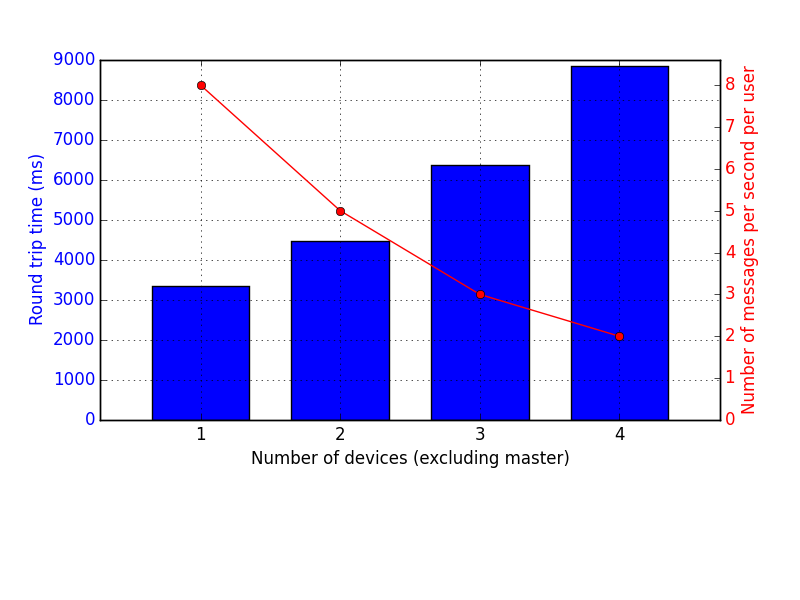
\includegraphics[width=1.0\textwidth]{img/messages_per_second.png} 
  \caption{Estimate of Round Trip Time and Messages per second rate}
  \label{figure:messages-per-second}
\end{figure}